\chapter{Model dyskretny}
Dla przyjętego czasu próbkowania Tp = 0.01 min.
\section{Równania stanu}
Wychodząc od równania stanu modelu ciągłego i wykorzystując obecną w Matlabie funkcję $c2d()$ otrzymaliśmy równania stanu modelu dyskretnego.
\begin{equation}
	\left\{
	\begin{tabular}{l}
	$C_A[k+1] = 0.9233\cdot C_A[k]  -0.0009228\cdot T[k]+ 0.009618\cdot C_{Ain}[k]+  2.811\cdot 10^{-5}\cdot F_C[k]$\\
	$\quad \quad -4.629\cdot 10^{-6}\cdot T_{in}[k]  -2.473\cdot 10^{-5}\cdot T_{Cin}[k]$\\\\
	$T[k+1] = 8.447\cdot C_A[k] +1.055\cdot T[k]+ 0.042378\cdot C_{Ain}[k]-0.06244\cdot F_C[k]$\\
	$\quad \quad +0.01028\cdot T_{in}[k]  +0.05492\cdot T_{Cin}[k]$\\
	\end{tabular}
	\right.
\end{equation}
\section{Transmitancja}
Mając transmitancję modelu ciągłego wykorzystaliśmy obecną w Matlabie funkcję $c2d()$ w celu otrzymania transmitancji modelu dyskretnego.
\begin{equation}
	\frac{C_A(z)}{C_{Ain}(z)} = \frac{0.009618z-0.01019}{z^2-1.979z+0.9823}
\end{equation}
\begin{equation}
\frac{C_A(z)}{F_C(z)} = \frac{2.811\cdot10^{-5}z-2.795\cdot10^{-5}}{z^2-1.979z+0.9823}
\end{equation}
\begin{equation}
\frac{C_A(z)}{T_{in}(z)} = \frac{-4.629\cdot10^{-6} z - 4.601\cdot10^{-6}}{z^2-1.979z+0.9823}
\end{equation}
\begin{equation}
\frac{C_A(z)}{T_{Cin}(z)} = \frac{-2.473\cdot10^{-5} z - 2.458\cdot 10^{-5}}{z^2-1.979z+0.9823}
\end{equation}
\begin{equation}
\frac{T(z)}{C_{Ain}(z)} = \frac{0.04237 z + 0.04212}{z^2-1.979z+0.9823}
\end{equation}
\begin{equation}
\frac{T(z)}{F_C(z)} = \frac{-0.06244 z + 0.05789}{z^2-1.979z+0.9823}
\end{equation}
\begin{equation}
\frac{T(z)}{T_{in}(z)} = \frac{0.01028 z - 0.009532}{z^2-1.979z+0.9823}
\end{equation}
\begin{equation}
\frac{T(z)}{T_{Cin}(z)} = \frac{0.05492 z - 0.05092}{z^2-1.979z+0.9823}
\end{equation}

Odpowiedzi skokowe modeli dyskretnych w postaci zarówno równań stanu jak i transmitancji wyglądają identycznie, co widać na wykresach \ref{fig:step_ss} oraz \ref{fig:step_tf}. Można dzięki temu wnioskować, że transmitancje zostały wyznaczone prawidłowo.

\begin{figure}
	\centering
	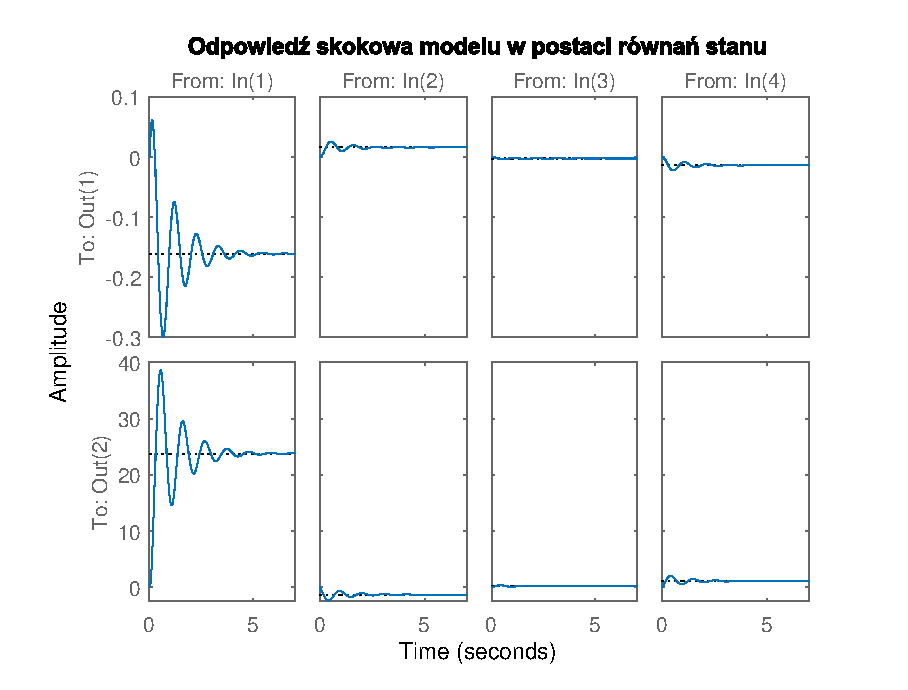
\includegraphics[width=.8\linewidth]{plot/step_space_state.eps}
	\caption{Odpowiedź skokowa modelu dyskretnego w postaci równań stanu}
	\label{fig:step_ss}
\end{figure}

\begin{figure}
	\centering
	\includegraphics[width=.8\linewidth]{plot/step_transfer.eps}
	\caption{Odpowiedź skokowa modelu dyskretnego w transmitancji}
	\label{fig:step_tf}
\end{figure}

\newpage
\section{Porównanie modelu dyskretnego i ciągłego}
Na poniższych wykresach (od \ref{fig:dys01} do \ref{fig:dys001}) porównaliśmy działanie modelu dyskretnego i ciągłego przy skokach obydwu sterowań dla trzech różnych okresów próbkowania: 0.1, 0.05 oraz 0.01 minuty. Dla największej z tych wartości dokładnie widać różnicę, między modelami, a mianowicie charakterystyczne schodki. Dla okresu 0.05 minuty schodki są jeszcze widoczne, ale wykres wygląda znacznie lepiej. Przy okresie próbkowania 0.01 minuty wykresy wykresy niemalże nakładają się na siebie, więc to właśnie tę wartość wybraliśmy jako optymalną.
\begin{figure}
	\centering
	\includegraphics[width=.8\linewidth]{plot/dysk_1.eps}
	\caption{Porównanie modelu ciągłego i dyskretnego dla czasu próbkowania 0.1 min}
	\label{fig:dys01}
\end{figure}
\begin{figure}
\centering
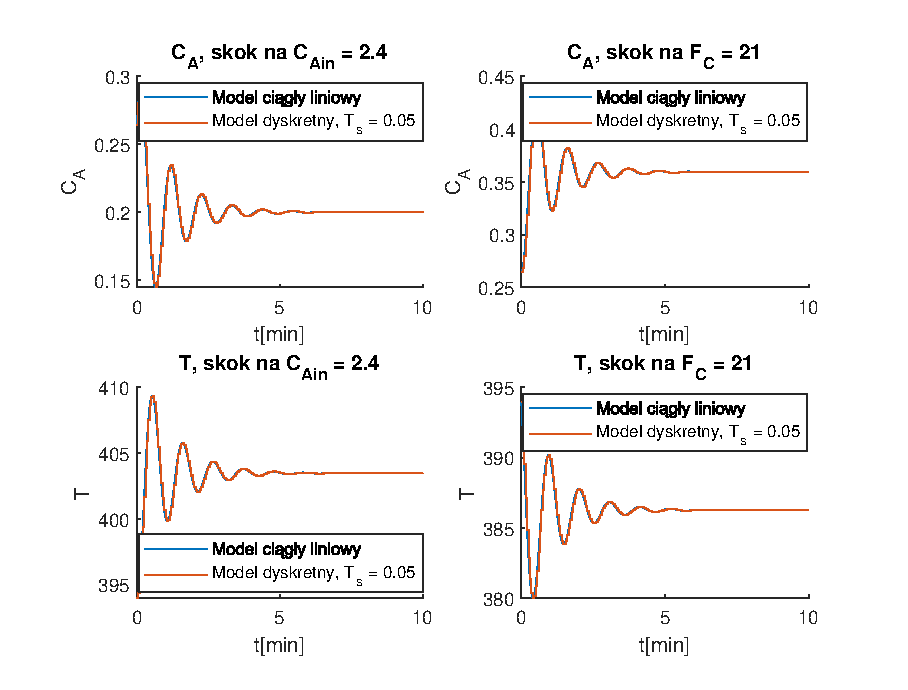
\includegraphics[width=.8\linewidth]{plot/dysk_05.eps}
\caption{Porównanie modelu ciągłego i dyskretnego dla czasu próbkowania 0.05 min}
\label{fig:dys005}
\end{figure}
\begin{figure}
\centering
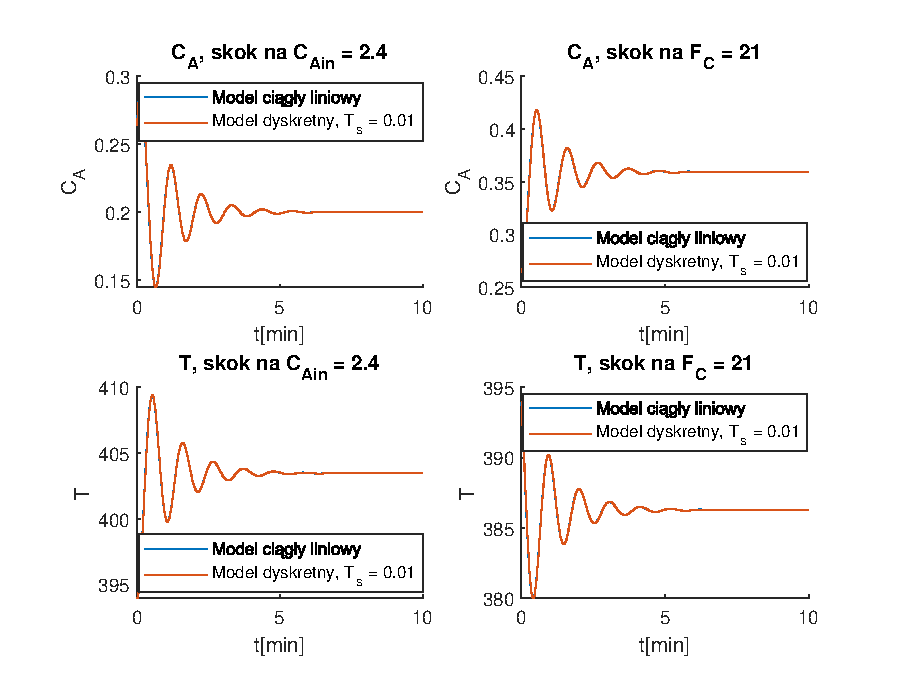
\includegraphics[width=.8\linewidth]{plot/dysk_01.eps}
\caption{Porównanie modelu ciągłego i dyskretnego dla czasu próbkowania 0.01 min}
\label{fig:dys001}
\end{figure}
